\chapter{Background}
This chapter aim to give the reader the necessary background to understand this
thesis.

\section{B.A.T.M.A.N.}
BATMAN \cite{batman_rfc} is an increasingly more popular routing protocol for
wireless ad hoc networks. The name is an abbreviation for ``Better Approach To
Mobile Ad hoc Networking''. The motivation behind BATMAN was to replace OLSR
\cite{why-starting-batman} because of the inherent difficulties that protocol
has. 

OLSR is a pro-active routing protocol, which means that participating nodes
regularly exchange routing information with each other. According to the BATMAN
developers the problem with OLSR is that every node in the network calculates
the whole routing path, which is a complex way to do it. In addition, if nodes
sit on different routing information this concept leads to routing loops and
heavy route flapping. The result is many patches to the protocol that defies
the protocol standard in order to make it more suitable.

The developers of BATMAN wanted to start with a clean slate and decided amongst
other things that each node should only know the next hop, i.e. the link-local
neighbor that is the path between itself and the destination. In many ways, what
they did was to make a simpler and easier to understand protocol. For instance,
the way BATMAN calculates the optimal route, i.e. the next jump, is by comparing
the number of routing messages it has received from each node and who was the
last sender.

The routing messages sent in BATMAN are called \acp{OGM}. Figure
\ref{fig:original_ogm} show the packet format with all header fields. The
\ac{OGM} format has changed since the \cite{batman_rfc} was published, but there
is no publication with the new packet format as of yet. The updated packet
format can be found on the project's web pages \url{http://www.open-mesh.org/}.

\begin{figure}[ht!]
	\centering
  	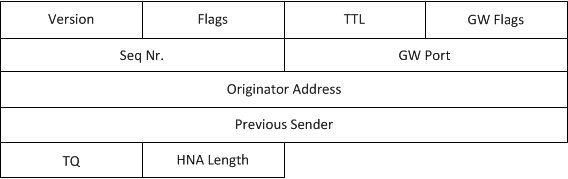
\includegraphics{images/original_ogm.png}
  	\caption{BATMAN's \acf{OGM} packet format.}
	\label{fig:original_ogm}
\end{figure}

The real workhorse of the packet is the ``Originator Address'' field which
carries the address of the node 'A' that sent out the \ac{OGM}. When a node 'B'
receives this message it checks if the originator address and source IP address
of the UDP header is the same - if so the two nodes are direct neighbors. B then
forwards the \ac{OGM} only changing the ``TTL'' and ``Previous Sender'' fields.
All \acp{OGM} are inside the BATMAN network is broadcasted like this until the
TTL has dropped to zero, or until they receive an \ac{OGM} they have
previously sent themselves.

This way all \acp{OGM} will be received and rebroadcasted by all nodes in the
network and all nodes will learn the existence of each other and which nodes are
the first jump between them and the other nodes, i.e. the first leg of the path.



\section{Proxy Certificates}

\section{Attacks on Mobile Ad Hoc Networks}
\subsection{Wormhole Attack}
\subsection{Blackhole Attack}
\subsection{Greyhole Attack}
